\documentclass[aspectratio=169, 11pt]{beamer}

% --- Packages & Setup ---
\usepackage[utf8]{inputenc}
\usepackage[T1]{fontenc}
\usepackage{xcolor}
\usepackage{booktabs}
\usepackage{graphicx}
\usepackage{tikz}
\usetikzlibrary{calc}

\graphicspath{{../}{./}}

% Try loading Open Sans; fallback if missing
\IfFileExists{opensans.sty}{\usepackage[default,scale=0.95]{opensans}}{}

% --- Branding Colors ---
\definecolor{amritaMaroon}{HTML}{A4123F}

% --- Theme Setup ---
\usetheme{Madrid}
\usecolortheme[named=amritaMaroon]{structure}
\setbeamertemplate{navigation symbols}{}
\setbeamertemplate{footline}[frame number]

\begin{document}

% --- CUSTOM TITLE SLIDE (Research) ---
\begin{frame}
    % Corner Box Indicator
    \begin{tikzpicture}[remember picture,overlay]
        \node[fill=amritaMaroon, text=white, font=\bfseries\footnotesize, anchor=north east, rounded corners=2pt, inner sep=5pt]
        at ($(current page.north east) + (-0.2cm,-0.2cm)$)
        {Type 1: Research Project};
    \end{tikzpicture}

    \centering
    \IfFileExists{logo.png}{\includegraphics[width=2.8cm]{logo.png}\vspace{0.1cm}}{\vspace{0.4cm}}

    {\large \textbf{\textcolor{amritaMaroon}{PORYGON: A Statistical and Rule-Based Runtime Security Framework for Containerized Workloads}}} \\
    \vspace{0.05cm}
    {\footnotesize \textbf{23CSE498 -- Project Phase 2 (Panel Review 1)} \quad | \quad \textbf{Team Number: 75}} \\
    \vspace{0.15cm}

    % Student Table
    \begin{table}
        \centering
        \footnotesize
        \renewcommand{\arraystretch}{1.05}
        \begin{tabular}{|c|c|l|}
            \hline
            \textbf{S.No} & \textbf{Register Number} & \textbf{Student Name} \\
            \hline
            1 & CB.EN.U4CSE23504 & Ashin Varghese \\
            \hline
            2 & CB.EN.U4CSE23559 & Anurup Krishna \\
            \hline
            3 & CB.EN.U4CSE23628 & Krishnan S \\
            \hline
            4 & CB.EN.U4CSE23661 & Madhav Sreejith \\
            \hline
        \end{tabular}
    \end{table}
    \vspace{0.1cm}

    {\footnotesize Guide: \textbf{Dr Abirami K}, Assistant Professor, Department of CSE} \\
    \vspace{0.1cm}
    {\scriptsize \today}
\end{frame}

% ============================================================
% RESEARCH QUESTION AND CONTRIBUTION
% ============================================================
\section{Research Question}
\begin{frame}{Research Question and Contribution}
\framesubtitle{The specific, falsifiable question this project answers}

\scriptsize
\textbf{System overview:} Porygon ingests Falco eBPF process-execution
events and Docker lifecycle events per container image digest, computes
the Jensen--Shannon distance between a versioned historical baseline and
the current runtime window, and correlates the resulting score against
seven deterministic detection rules. A match produces a finding gated by
explicit severity/confidence thresholds; no containment action executes
without human operator approval.

\smallskip
\textbf{The unanswered design question:} container security tools learn
what ``normal'' process behavior looks like, then flag deviations. But how
finely should ``normal'' be defined? Four real options, in increasing
order of specificity:

\begin{enumerate}
\setlength{\itemsep}{1pt}
\item \textbf{One-size-fits-all} -- a single baseline shared by every
container regardless of what image it runs.
\item \textbf{Per mutable label} -- one baseline per image tag (e.g.
\texttt{myapp:latest}); the risk is that a tag can be silently repointed to
different image content later.
\item \textbf{Per exact image} -- one baseline per cryptographic image
identity, which cannot silently change.
\item \textbf{Per exact image + configuration} -- the same, but also
split by the container's specific security settings (permissions,
capabilities).
\end{enumerate}

No existing tool or published study (Falco, Sysdig, Aqua, or the academic
line from Forrest et al. 1996 through Abed/Clancy 2015) measures which of
these four actually reduces false alarms. This project does, using 216
real container trials and formal statistical testing rather than a single
accuracy figure.

\smallskip
\textbf{Result:} option 3 eliminated false alarms entirely versus option 1
($100\%\to0\%$), without missing any real attack (96/96 caught either
way). This was not a fluke -- the same result appeared at two different
sample sizes ($p=5.8\times10^{-11}$ at 144 trials, $p=6.7\times10^{-16}$
at 216 trials), and got statistically stronger, not weaker, the second
time.
\end{frame}

% --- NOVELTY / UNIQUENESS ---
\section{Novelty}
\begin{frame}{Novelty and Positioning Against Prior Work}
\framesubtitle{What is actually new here, stated precisely}
\scriptsize

\textbf{What is not new:} eBPF-based container process monitoring
and Jensen--Shannon divergence as a distance measure (Lin 1991; Salem \&
Na\"it-Abdesselam, ICC 2012, network traffic) both predate this project.

\medskip
\textbf{What is new:} no located tool or published study -- commercial
(Falco, Sysdig, Aqua) or academic (Forrest 1996 through 2025--2026) --
measures which of four concrete baseline-scoping granularities (pooled /
mutable-tag / exact-digest / digest-plus-configuration) actually reduces
false alarms, using controlled trials and significance testing rather
than a single accuracy figure. This project runs that comparison and
reports both a significant result and a null result from one protocol.

\medskip
\textbf{Closest prior work, checked directly:}
\begin{itemize}
    \setlength{\itemsep}{1pt}
    \item Abed, Clancy \& Levy (GLOBECOM Workshops, 2015) -- closest match:
    container-level, kernel-observed, no-prior-knowledge detection. Uses
    bag-of-syscalls, not JS-distance; no scoping comparison.
    \item Lin et al., ``eBPF-Guard'' (\emph{Empirical Software Engineering},
    Dec 2025) -- same sensor layer, scores via a fine-tuned LLM; single
    99.22\% accuracy figure, no scoping comparison.
    \item Li/Yuan/Wu/Cheng (2025) and Xiong/Wu/Jia, ``DeepContainer''
    (2025) -- neural container anomaly detectors, single point-estimate
    accuracy (96.8--99\%), no confidence interval or significance test.
\end{itemize}
All independently verified (DOI resolution or direct publisher fetch);
full list in \texttt{docs/RELATED\_WORK\_RECENT.md}.
\end{frame}

% --- ARCHITECTURE ---
\begin{frame}{System Architecture}
\framesubtitle{Eight containerized services, three network segments}
\begin{columns}[T,onlytextwidth]
\column{0.56\textwidth}
\scriptsize
\begin{itemize}
    \setlength{\itemsep}{2pt}
    \item \textbf{falco} -- eBPF driver; captures \texttt{execve} and
    lifecycle events at the kernel boundary.
    \item \textbf{collector} -- reads Docker daemon events; SQLite
    outbox with retry delivery.
    \item \textbf{telemetry} -- ingests Falco process-execution events,
    same outbox pattern.
    \item \textbf{backend} -- baseline construction, JSD scoring,
    seven-rule detection engine, response-policy logic.
    \item \textbf{scanner} -- Trivy CycloneDX SBOM generation, EPSS and
    CISA KEV enrichment.
    \item \textbf{responder} -- executes approved containment actions
    only after explicit human approval.
    \item \textbf{gateway} -- single ingress point for API and dashboard.
    \item \textbf{postgres} -- durable store for events, baselines,
    scores, findings, incidents, scan results.
\end{itemize}
\column{0.42\textwidth}
\scriptsize
\textbf{Network segregation (\texttt{compose.yaml}):}
\begin{itemize}
    \setlength{\itemsep}{2pt}
    \item \texttt{porygon\_ingress} -- external-facing traffic only
    (gateway).
    \item \texttt{porygon\_internal} -- inter-service communication.
    \item \texttt{porygon\_egress} -- outbound-only, granted exclusively
    to the scanner.
\end{itemize}
\medskip
A service outside a segment has no network path to it; the scanner is
the only service with outbound internet reachability.
\end{columns}
\end{frame}

% --- SLIDE 1: METHODOLOGY & SOLUTION DESIGN (Rubric: 5 Marks) ---
\section{Methodology \& Solution Design}

\begin{frame}{1. Methodology \& Solution Design}
    \framesubtitle{Rubric: Methodology, Implementation Approach \& Design Choices (5 Marks)}

    \begin{columns}[T,onlytextwidth]
        \column{0.48\textwidth}
        \footnotesize
        \textbf{Methodological Framework:}
        \setlength{\abovedisplayskip}{4pt}
        \setlength{\belowdisplayskip}{4pt}

        \begin{itemize}
            \setlength{\itemsep}{5pt}

            \item \textbf{Behaviour Baseline:}
            Historical Docker lifecycle and Falco process events form a
            versioned baseline for one immutable image digest.

            \item \textbf{Anomaly Scoring:}
            For each categorical feature, the v1 scorer compares baseline $P$
            with a completed runtime window $Q$ using base-2 Jensen--Shannon
            \emph{distance} (the square root of the Jensen--Shannon
            \emph{divergence}, bounded in $[0,1]$):
            \[
                D_{\mathrm{JS}}(P,Q) = \sqrt{\mathrm{JSD}(P,Q)},
                \quad
                \mathrm{JSD}(P,Q) = \tfrac{1}{2}D_{\mathrm{KL}}(P\|M) + \tfrac{1}{2}D_{\mathrm{KL}}(Q\|M),
                \quad M = \tfrac{1}{2}(P+Q)
            \]
            Smaller values indicate more similar behaviour.

            \item \textbf{Rule-Based Detection:}
            Seven deterministic rules produce explainable findings. An incident
            requires an unsuppressed, incident-eligible finding.
        \end{itemize}

        \column{0.48\textwidth}
        \centering
        {\small\textbf{Porygon Workflow}}\par
        \vspace{2mm}

        \begingroup

        \sbox{0}{%
        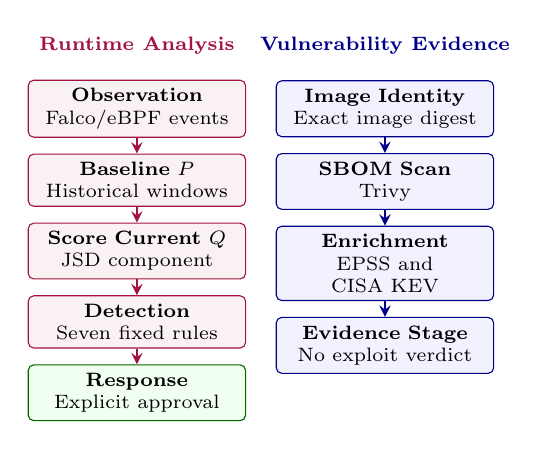
\begin{tikzpicture}[
            runtimebox/.style={
                draw=amritaMaroon,
                fill=amritaMaroon!6,
                rounded corners=2pt,
                text width=2.55cm,
                minimum height=0.65cm,
                inner sep=3pt,
                align=center,
                font=\scriptsize
            },
            evidencebox/.style={
                runtimebox,
                draw=blue!55!black,
                fill=blue!5
            },
            responsebox/.style={
                runtimebox,
                draw=green!40!black,
                fill=green!6
            },
            runtimearrow/.style={
                ->,
                >=stealth,
                thick,
                draw=amritaMaroon
            },
            evidencearrow/.style={
                runtimearrow,
                draw=blue!55!black
            }
        ]

        % --- Runtime analysis ---
        \node[runtimebox] (monitor) at (0,0)
            {\textbf{Observation}\\Falco/eBPF events};

        \node[
            font=\scriptsize\bfseries,
            text=amritaMaroon,
            anchor=south
        ] at ([yshift=2mm]monitor.north)
            {Runtime Analysis};

        \node[runtimebox, anchor=north]
            (baseline) at ([yshift=-2mm]monitor.south)
            {\textbf{Baseline $P$}\\Historical windows};

        \node[runtimebox, anchor=north]
            (score) at ([yshift=-2mm]baseline.south)
            {\textbf{Score Current $Q$}\\JSD component};

        \node[runtimebox, anchor=north]
            (detect) at ([yshift=-2mm]score.south)
            {\textbf{Detection}\\Seven fixed rules};

        \node[responsebox, anchor=north]
            (respond) at ([yshift=-2mm]detect.south)
            {\textbf{Response}\\Explicit approval};

        \draw[runtimearrow] (monitor.south) -- (baseline.north);
        \draw[runtimearrow] (baseline.south) -- (score.north);
        \draw[runtimearrow] (score.south) -- (detect.north);
        \draw[runtimearrow] (detect.south) -- (respond.north);

        % --- Vulnerability evidence ---
        \node[evidencebox] (digest) at (3.15,0)
            {\textbf{Image Identity}\\Exact image digest};

        \node[
            font=\scriptsize\bfseries,
            text=blue!55!black,
            anchor=south
        ] at ([yshift=2mm]digest.north)
            {Vulnerability Evidence};

        \node[evidencebox, anchor=north]
            (scan) at ([yshift=-2mm]digest.south)
            {\textbf{SBOM Scan}\\Trivy};

        \node[evidencebox, anchor=north]
            (enrich) at ([yshift=-2mm]scan.south)
            {\textbf{Enrichment}\\EPSS and CISA KEV};

        \node[evidencebox, anchor=north]
            (stage) at ([yshift=-2mm]enrich.south)
            {\textbf{Evidence Stage}\\No exploit verdict};

        \draw[evidencearrow] (digest.south) -- (scan.north);
        \draw[evidencearrow] (scan.south) -- (enrich.north);
        \draw[evidencearrow] (enrich.south) -- (stage.north);

        \end{tikzpicture}%
        }

        \ifdim\wd0>\linewidth
            \sbox{0}{\resizebox{\linewidth}{!}{\usebox{0}}}%
        \fi

        \ifdim\dimexpr\ht0+\dp0\relax>0.50\paperheight
            \resizebox*{!}{0.50\paperheight}{\usebox{0}}%
        \else
            \usebox{0}%
        \fi

        \par
        \endgroup
    \end{columns}
\end{frame}

\begin{frame}{1. Methodology \& Solution Design (contd.)}
    \framesubtitle{Rubric: Methodology, Implementation Approach \& Design Choices (5 Marks)}

    \footnotesize
    \textbf{Implementation Approach and Design Choices:}

    \begin{itemize}
        \setlength{\itemsep}{7pt}

        \item \textbf{Kernel-Level Monitoring:}
        Falco's modern eBPF driver captures container process execution without
        modifying the applications. The Telemetry Adapter ingests those events,
        while the Docker Collector records lifecycle and image-identity events.
        Both use bounded SQLite outboxes with retry delivery.

        \item \textbf{Service Integration:}
        Docker Compose coordinates eight long-running containers. Segregated
        networks restrict connectivity, and outbound access is limited to the
        vulnerability scanner.

        \item \textbf{Explainable Analysis:}
        Base-2 Jensen--Shannon distance provides a bounded, symmetric measure of
        categorical change. Fixed rules expose the matched evidence, so the
        implemented path does not depend on a black-box ML classifier.

        \item \textbf{Controlled Response:}
        Policy thresholds use severity and confidence to determine allowed
        containment actions. Disruptive execution is disabled by default. When
        enabled, it still requires explicit human approval.

        \item \textbf{Implementation Verification:}
        The repository contains 79 backend test functions across baseline,
        scoring, detection, calibration, response, and vulnerability modules,
        plus 131 further test functions across the collector, telemetry,
        responder, and scanner services (210 total).
    \end{itemize}
\end{frame}


% --- SLIDE 2: IMPLEMENTATION PROGRESS (Rubric: 8 Marks) ---
\section{Implementation Progress}
\begin{frame}{2. Implementation Progress \& Module Functionality}
    \framesubtitle{Rubric: Core Modules Implemented, Functional \& Integrated (8 Marks)}
    \begin{itemize}
        \item \textbf{Implementation Status Overview:}
    \end{itemize}
    \begin{table}
        \centering
        \small
        \renewcommand{\arraystretch}{1.15}
        \begin{tabular}{|p{4.2cm}|p{5.8cm}|c|}
            \hline
            \textbf{Module / Component} & \textbf{Current Implementation State} & \textbf{Status} \\
            \hline
            Kernel Telemetry \& Ingestion (Falco eBPF, Docker Collector, Telemetry Adapter) & Captures container process execution via eBPF; durable SQLite outbox with retry & Functional \\
            \hline
            Behavioural Baseline \& JSD Scoring (\texttt{baseline.py}, \texttt{scoring.py}) & Digest-bound behavioural baselines; JSD-based anomaly distance scoring & Functional \\
            \hline
            Deterministic Detection Engine (\texttt{detection.py}) & 7 correlation rules (POR-DET-001--007) generating findings/incidents & Functional \\
            \hline
            4-Arm Scope Comparison (\texttt{experiments/}) & 216-trial confirmatory run analysed end to end, exact statistical pipeline & Complete \\
            \hline
        \end{tabular}
    \end{table}
\end{frame}

\begin{frame}{2. Implementation Progress (contd.)}
    \framesubtitle{Rubric: Core Modules Implemented, Functional \& Integrated (8 Marks)}
    \begin{table}
        \centering
        \small
        \renewcommand{\arraystretch}{1.15}
        \begin{tabular}{|p{4.2cm}|p{5.8cm}|c|}
            \hline
            \textbf{Module / Component} & \textbf{Current Implementation State} & \textbf{Status} \\
            \hline
            Vulnerability \& SBOM Pipeline (Scanner, Trivy 0.72.0) & CycloneDX SBOM generation; EPSS \& CISA KEV enrichment & Functional \\
            \hline
            Response Policy Engine (\texttt{response.py}) & Severity/confidence-gated containment recommendations; human-approval required & Functional \\
            \hline
            Module Integration & 8 containerized services integrated via Docker Compose with network segregation & Integrated \\
            \hline
        \end{tabular}
    \end{table}
    \vspace{0.3cm}
    \footnotesize \textbf{Core Functionality Demonstration:} A real, functional
    XMRig cryptominer binary from a published malware-sample container image
    was executed against a live Porygon baseline built from 243 real
    Falco-captured events, with zero prior knowledge of the binary given to
    the system. Resulting anomaly score: 0.2696 (\texttt{elevated} band,
    threshold 0.25), with the executable and its parent-child call edge both
    flagged as previously unseen. Full record: \texttt{docs/LIVE\_DEMO\_RECORD\_V1.md}.
\end{frame}

% --- LIVE TEST RESULTS AND COMPARISON ---
\begin{frame}{Live Test Results and Comparison}
\framesubtitle{Confirmatory statistical run (216 trials) alongside the live malware demonstration}
\scriptsize
\begin{table}
    \centering
    \scriptsize
    \renewcommand{\arraystretch}{1.1}
    \begin{tabular}{|l|c|c|}
        \hline
        \textbf{Baseline arm} & \textbf{FPR (benign, n=53)} & \textbf{Recall (attacks, n=96)} \\
        \hline
        ARM-GLOBAL (pooled, one baseline for all) & 100\% [93.3--100\%] & 100\% \\
        \hline
        ARM-TAG (per mutable image tag) & 0\% [0--6.7\%] & 100\% \\
        \hline
        ARM-DIGEST (per exact image digest) & 0\% [0--6.7\%] & 100\% \\
        \hline
        ARM-CONTEXT (digest + runtime config) & 0\% [0--6.7\%] & 100\% \\
        \hline
    \end{tabular}
\end{table}
\vspace{-2mm}
CONTEXT vs.\ GLOBAL: $p=6.7\times10^{-16}$ (significant). CONTEXT vs.\
DIGEST, the harder comparison this project's thesis rests on: $p=1.0$
(null, arms agree on all 53 held-out trials -- reported as-is).

\medskip
\textbf{Independent live test (not part of the 216-trial protocol):} a
real XMRig cryptominer binary, from a published malware-testing container
image, executed against a Porygon baseline built from 243 genuinely
captured Falco events, scorer given no prior knowledge of the binary.
\begin{itemize}
    \setlength{\itemsep}{1pt}
    \item Anomaly scorer: flagged, score 0.2696 (\texttt{elevated} band,
    threshold 0.25) -- correct detection with zero prior signature.
    \item Deterministic rule POR-DET-004: did \emph{not} fire --
    \texttt{xmrig} is absent from its hardcoded dual-use-tool list, a
    real, disclosed gap.
\end{itemize}
Full record: \texttt{docs/LIVE\_DEMO\_RECORD\_V1.md}.
\end{frame}

% --- DETECTION RULES DETAIL ---
\begin{frame}{Deterministic Detection Rules (\texttt{detection.py})}
\framesubtitle{Seven fixed rules producing explainable findings}
\centering
\tiny
\renewcommand{\arraystretch}{1.3}
\begin{tabular}{|l|p{7.8cm}|c|c|c|}
    \hline
    \textbf{Rule} & \textbf{Trigger condition} & \textbf{Sev.} & \textbf{Conf.} & \textbf{Inc.} \\
    \hline
    POR-DET-001 & Completed window scores $\geq 0.50$ behavioural distance & 0.65 & 0.70 & No \\
    \hline
    POR-DET-002 & Shell executable absent from the digest baseline executed & 0.72 & 0.90 & Yes \\
    \hline
    POR-DET-003 & UID 0 process executed with UID 0 absent from baseline & 0.78 & 0.90 & Yes \\
    \hline
    POR-DET-004 & Downloader/network/interpreter/encoding tool absent from baseline & 0.64 & 0.80 & Yes \\
    \hline
    POR-DET-005 & Unseen shell followed by unseen dual-use tool, same window & 0.90 & 0.95 & Yes \\
    \hline
    POR-DET-006 & Docker exec activity during the observation window & 0.35 & 0.95 & No \\
    \hline
    POR-DET-007 & Container reported privileged mode during the window & 0.92 & 0.95 & Yes \\
    \hline
\end{tabular}
\par
\vspace{2mm}
\raggedright
\scriptsize
An incident requires at least one \emph{incident-eligible} finding;
POR-DET-001 and POR-DET-006 alone never open an incident, they only
contribute evidence. Severity/confidence weights are fixed constants in
source, not tuned per deployment.
\end{frame}


% --- SLIDE 3: TECHNICAL KNOWLEDGE & DESIGN CHOICES (Rubric: 5 Marks) ---
\section{Technical Knowledge}
\begin{frame}{3. Technical Knowledge \& Design Decisions}
    \framesubtitle{Rubric: Understanding of Methodology, Implementation \& Design Choices (5 Marks)}
    \footnotesize

    \textbf{Distance metric selection: Jensen-Shannon divergence (JSD) over
    Kullback-Leibler (KL) divergence.} KL divergence is asymmetric
    ($D_{KL}(P,Q)\neq D_{KL}(Q,P)$) and unbounded above, so a KL score
    computed for one container cannot be compared against a KL score from a
    different container on a common scale. JSD is the symmetric, bounded
    variant ($JSD(P,Q)=JSD(Q,P)$, range $[0,1]$), which permits one fixed
    threshold to apply uniformly across all containers.

    \medskip
    \textbf{Containment decision logic.} A finding does not trigger any
    action unless the rule engine's severity ($Sev$) and confidence
    ($Conf$) scores clear a defined threshold. Pause requires
    $Sev\geq0.70$ and $Conf\geq0.55$. Stop requires $Sev\geq0.90$,
    $Conf\geq0.75$, and a match on one of two specific high-confidence
    rules (unseen-shell-to-tool sequence, or a container transitioning to
    privileged mode). Every action, at either threshold, requires explicit
    human operator approval before execution; no threshold triggers
    automatic execution.

    \medskip
    \textbf{Statistical significance of the primary result.} On 216 real
    container trials, per-image baseline scoping reduced the false-alarm
    rate from 100\% to 0\% relative to a single pooled baseline, with zero
    reduction in attack detection. The exact statistical test applied to
    this result returns $p=6.7\times10^{-16}$, several orders of magnitude
    below the conventional $p<0.05$ significance threshold.
\end{frame}

\begin{frame}{3. Technical Knowledge \& Design Decisions (contd.)}
    \framesubtitle{Rubric: Understanding of Methodology, Implementation \& Design Choices (5 Marks)}
    \footnotesize

    \textbf{Multicall binary handling.} Utilities such as BusyBox and
    Toybox implement dozens of commands inside a single executable file;
    the command executed depends on the invocation name, not the file
    path. Tracking file identity alone would classify every invoked
    command as the same previously-seen program. The detection engine
    instead tracks the invocation (command) name, so a new command
    invoked through an already-known multicall binary is still flagged
    as novel.

    \medskip
    \textbf{Canonical scan identity.} Each vulnerability scan result is
    keyed by a SHA-256 hash of six inputs: image digest, local image ID,
    scanner name, scanner version, vulnerability database schema version,
    and a researcher-supplied scan reference. Re-executing a scan with an
    identical set of these six inputs returns the existing stored result
    (idempotent). A change to any one input produces a distinct,
    separately-tracked scan record (immutable).

    \medskip
    \textbf{Network segregation.} The eight services are partitioned
    across three isolated Docker networks: ingress (external traffic),
    internal (inter-service communication), and egress (outbound-only,
    used exclusively by the vulnerability scanner). A service is not
    granted network reachability to segments outside its assigned role.

    \medskip
    \textbf{Versioned scoring configuration.} The scoring algorithm and
    its numeric weights are bound to a named algorithm version. A weight
    modification requires incrementing the version identifier; no weight
    change is applied in place. Every historical score therefore remains
    reproducible against the exact configuration that produced it.
\end{frame}

\begin{frame}{3. Technical Knowledge \& Design Decisions (contd.)}
    \framesubtitle{Rubric: Understanding of Methodology, Implementation \& Design Choices (5 Marks)}
    \footnotesize
    \begin{itemize}
        \item \textbf{Confirmed Findings (216 real trials, exact statistical pipeline):}
        \begin{itemize}
            \item Per-image scoping vs.\ pooled baseline: significant, $p=6.7\times10^{-16}$, FPR $100\%\to0\%$, recall unchanged (96/96 both arms).
            \item Digest-plus-context vs.\ digest-only: no measurable difference in this dataset ($p=1.0$, expected here since the two arms produced identical confusion-matrix counts -- not a reporting error), reproduced at both $n=35$ and $n=53$ -- traced to the tested configuration change (a dropped Linux capability) not altering which processes execute, which the process-name feature cannot see by construction.
            \item Follow-on feature scoring the security-configuration document directly separates every tested case cleanly: 0/26 false positives, 27/27 correct detections.
        \end{itemize}
    \end{itemize}
\end{frame}

% --- ADVERSARIAL SCENARIOS / THREAT MODEL ---
\begin{frame}{Adversarial Scenario Analysis}
\framesubtitle{18 scenarios classified against the actual implementation, not asserted}
\scriptsize
\begin{itemize}
    \setlength{\itemsep}{3pt}
    \item \textbf{Structurally invisible (6 of 18):} attacks reusing an
    already-baselined process, adding no new \texttt{execve} event -- C2
    domain repoint, exfiltration over an existing channel, file-only
    webshell, DNS tunnelling, fileless execution, payload inside an
    already-baselined HTTPS request. No syscall-argument or network
    telemetry exists in v1; explicitly out of scope in
    \texttt{THREAT\_MODEL\_V1.md}, not a hidden gap.

    \item \textbf{Depends on process-identity granularity (4 of 18):}
    in-place binary replacement keeping the same path/name is likely
    invisible (identity tracked by name/path, not content hash); SUID
    privilege escalation to UID 0 \emph{is} caught (POR-DET-003).

    \item \textbf{Untested failure modes (3 of 18):} baseline poisoning
    during the fit window (defended by design, but the human-review step
    itself never exercised); low-and-slow attacks beyond the 120s
    correlation window; process-sequence-bigram mimicry. All three named
    directly in the project's own threat model.

    \item \textbf{Where the design genuinely helps (5 of 18):} backdoored
    entrypoint script (POR-DET-002); manual \texttt{docker exec}
    (POR-DET-006); flip to \texttt{--privileged} (POR-DET-007);
    mutable-tag digest substitution (digest scoping only); classic
    \texttt{curl | bash} dropper pattern (POR-DET-005, confidence 0.95).
\end{itemize}
Full scenario-by-scenario table: \texttt{docs/ADVERSARIAL\_SCENARIOS\_V1.md}.
\end{frame}

% --- VERIFICATION AND TESTING RIGOR ---
\begin{frame}{Verification and Testing Rigor}
\framesubtitle{How correctness of the claimed results is actually checked}
\scriptsize
\begin{itemize}
    \setlength{\itemsep}{3pt}
    \item \textbf{Layered verification (\texttt{scripts/verify\_all.sh}):}
    \texttt{static} (lint/type checks), \texttt{unit} (210 backend and
    service test functions), \texttt{live-safe} (non-disruptive real
    Docker container checks), \texttt{scanner-live}/\texttt{experiment-live}
    (pinned-digest real-container acceptance tests) -- separate
    \texttt{make} targets, none mocked end-to-end.

    \item \textbf{Frozen protocol before results:} the statistical
    protocol (\texttt{porygon.research.protocol.v1}) was written and
    reviewed \emph{before} the confirmatory run, with a pre-registered
    sample size, primary contrast, and material-effect threshold, marked
    \texttt{FROZEN} -- cannot be edited post hoc to fit a result.

    \item \textbf{Six real bugs found and fixed} to obtain the first
    confirmatory result: a wrong API field name silently blocking all
    detections, dead code blocking attack scenarios, a fit-reference
    contamination bug, and an infinite-recursion bug in the
    Clopper--Pearson confidence-interval code itself. Commit range in
    \texttt{CONFIRMATORY\_RESULT\_V1.md}.

    \item \textbf{Reproducibility:} every reported number has a named
    artifact path and a documented reproduce command.

    \item \textbf{Disclosed limitation:} single-reviewer self-review, not
    independent third-party peer review -- stated plainly.
\end{itemize}
\end{frame}

% --- TEAM CONTRIBUTION AND PROJECT STATUS ---
\begin{frame}{Team Contribution and Project Status}
\framesubtitle{Phase 2 deliverables against the original scope}
\scriptsize
\begin{table}
    \centering
    \scriptsize
    \renewcommand{\arraystretch}{1.05}
    \begin{tabular}{|p{4.7cm}|p{6.3cm}|}
        \hline
        \textbf{Deliverable} & \textbf{State at this review} \\
        \hline
        eBPF/Falco telemetry pipeline & Functional, integrated, durable outbox delivery \\
        \hline
        Baseline + JSD scoring engine & Functional, versioned configuration \\
        \hline
        7-rule deterministic detection & Functional, POR-DET-001--007 \\
        \hline
        Vulnerability/SBOM enrichment & Functional, Trivy + EPSS + CISA KEV \\
        \hline
        Response policy engine & Functional, human-approval gated \\
        \hline
        4-arm scoping confirmatory study & Complete, 216 trials, two reproduced results \\
        \hline
        Live real-malware demonstration & Complete, XMRig, documented including the miss \\
        \hline
        Independent literature verification & Complete, 10 papers checked by DOI/API/direct fetch \\
        \hline
    \end{tabular}
\end{table}
All eight modules are integrated into one running Docker Compose stack
(\texttt{make up}) and independently exercised through
\texttt{scripts/verify\_all.sh}, not demonstrated in isolation.
\end{frame}

% --- SLIDE 4: TECHNICAL ENRICHMENT ACTIVITY CHOICES ---
\section{Technical Enrichment}
\begin{frame}{4. Technical Enrichment Activity Choices}
    \framesubtitle{Professional Online Certification Details (Individual Mandatory: 10--20 Hours)}
    \begin{itemize}
        \item \textbf{Individual MOOC / Online Certification Selection:}
    \end{itemize}
    \vspace{-0.1cm}
    \begin{table}
        \centering
        \footnotesize
        \renewcommand{\arraystretch}{1.15}
        \begin{tabular}{|c|p{2.8cm}|p{5.5cm}|p{1.8cm}|c|}
            \hline
            \textbf{S.No} & \textbf{Student Name} & \textbf{Chosen MOOC / Course Title} & \textbf{Platform} & \textbf{Hours} \\
            \hline
            1 & Ashin Varghese & Introduction to Kubernetes (LFS158) & edX & 15 Hrs \\
            \hline
            2 & Anurup Krishna & Introduction to Kubernetes (LFS158) & edX & 20 Hrs \\
            \hline
            3 & Krishnan S & Introduction to Kubernetes (LFS158) & edX & 12 Hrs \\
            \hline
            4 & Madhav Sreejith & Introduction to Kubernetes (LFS158) & edX & 16 Hrs \\
            \hline
        \end{tabular}
    \end{table}
    \vspace{0.15cm}
    \begin{itemize}
        \item {\scriptsize \textbf{Requirement:} Each student must complete one approved 10--20 hour online certification from a recognized platform (Coursera, NPTEL, edX, etc.) relevant to the project.}
    \end{itemize}
\end{frame}

% --- LIMITATIONS & FUTURE WORK ---
\section{Limitations \& Future Work}
\begin{frame}{Limitations \& Future Work}
\footnotesize

\textbf{Limitations:}
\begin{itemize}
    \item The confirmatory 216-trial run covers the tested attack and
    workload set; it does not claim coverage of every real-world attack
    pattern or benign workload shape.
    \item Scoring uses categorical process-name/edge features; it does not
    yet model syscall argument content or network payloads.
    \item Response actions require a human operator in the loop by design
    -- there is no fully autonomous containment path.
\end{itemize}

\medskip
\textbf{Future Work:}
\begin{itemize}
    \item Extend the per-image + configuration baseline to a larger,
    more diverse container corpus beyond the 216-trial dataset.
    \item Evaluate additional distance metrics and richer feature sets
    (e.g. syscall arguments) against the same statistical protocol.
    \item Explore semi-automated response for the highest-confidence
    rule matches, still gated by policy and audit logging.
\end{itemize}
\end{frame}

% --- REFERENCES ---
\section{References}
\begin{frame}[allowframebreaks]{References}
\scriptsize
\begin{thebibliography}{9}

\bibitem{forrest1996}
S.~Forrest, S.~A. Hofmeyr, A.~Somayaji, and T.~A. Longstaff,
``A sense of self for Unix processes,''
in \emph{Proc. IEEE Symp. Security and Privacy}, 1996, pp.~120--128.

\bibitem{hofmeyr1998}
S.~A. Hofmeyr, S.~Forrest, and A.~Somayaji,
``Intrusion detection using sequences of system calls,''
\emph{Journal of Computer Security}, vol.~6, no.~3, pp.~151--180, 1998.

\bibitem{abed2015}
A.~S. Abed, T.~C. Clancy, and D.~S. Levy,
``Applying bag of system calls for anomalous behavior detection of applications
in Linux containers,''
in \emph{Proc. IEEE Globecom Workshops}, 2015, pp.~1--5.

\bibitem{lin1991}
J.~Lin,
``Divergence measures based on the Shannon entropy,''
\emph{IEEE Trans. Information Theory}, vol.~37, no.~1, pp.~145--151, 1991.

\bibitem{salem2012}
A.~Salem and F.~Naït-Abdesselam,
``Anomaly detection in network traffic using Jensen-Shannon divergence,''
in \emph{Proc. IEEE International Conference on Communications (ICC)}, 2012.

\bibitem{lin2026}
X.~Lin, Z.~Chen, W.~Yang, X.~Yang, J.~Luo, and X.~Yang,
``eBPF-Guard: a detection method for container escape via multi-level
monitoring and enhanced analysis model,''
\emph{Empirical Software Engineering}, vol.~31, article~51, 2026.

\bibitem{li2025}
Li Wei, Yuan Zekun, Wu Kehe, and Cheng Rui,
``Container anomaly detection based on attention mechanism and multiscale
convolutional neural network,''
\emph{Journal of Information Security Research}, vol.~11, no.~1, pp.~35--, 2025.

\bibitem{xiong2025}
K.~Xiong, Z.~Wu, and X.~Jia,
``DeepContainer: a deep learning-based framework for real-time anomaly
detection in cloud-native container environments,''
\emph{Journal of Advanced Computing Systems}, 2025.

\bibitem{ring2021}
J.~H. Ring, C.~M. Van Oort, S.~Durst, V.~White, J.~P. Near, and C.~Skalka,
``Methods for host-based intrusion detection with deep learning,''
\emph{Digital Threats: Research and Practice}, vol.~2, no.~4, 2021.

\bibitem{gregg2019}
B.~Gregg,
\emph{BPF Performance Tools: Linux System and Application Observability}.
Boston, MA, USA: Addison-Wesley, 2019.

\bibitem{falco}
The Falco Authors,
``Falco: cloud-native runtime security,''
Cloud Native Computing Foundation. [Online]. Available: https://falco.org

\bibitem{ociimage}
Open Container Initiative,
``OCI image format specification.'' [Online].
Available: https://github.com/opencontainers/image-spec

\end{thebibliography}
\end{frame}

% --- THANK YOU ---
\begin{frame}
    \centering
    {\Huge \textbf{\textcolor{amritaMaroon}{Thank You}}}
\end{frame}

\end{document}
